\chapter{Related work}
\label{chap:related}

In this chapter the related work regarding disparity algorithms is treated.
As integration of some disparity algorithms for the later evaluation was part of this thesis, the ones which were actually implemented are examined in more detail.
The well-known semi-global matcher by \citeauthor{hirschmuller2005accurate} is introduced and the OpenCV implementations are mentioned.
An approach by \citeauthor{Geiger2010ACCV} to enable fast matching of high-resolution images is discussed.
Both approaches utilize local methods for estimating disparity maps.
One candidate adopting global methods is the Middlebury MRF library, which is also introduced in this chapter.
This implies solving optimization problems (i.e. the minimization of a global energy cost function).
Thus, the methods implemented by the library to solve such optimization problems are outlined.
In the end, a short outlook on spatiotemporal consistency regarding disparity algorithms applied on videos is presented.

\section{Semi-global matching}

\citeauthor{hirschmuller2005accurate} combines two different methods, global- and local-matching for determining accurate disparity at a lower runtime as other global algorithms, which tend to run pretty long on current hardware \citep{hirschmuller2005accurate, hirschmuller2008stereo}.
\newline\newline\noindent The semi-global matching (SGM) method utilizes pixel-wise matching of so called mutual information (MI) via entropy $H$, their joint-entropy of a pair of images and combining those with the approximation of a global two-dimensional smoothness constraint:

\begin{equation}
  MI_{I_1,I_2} = H_{I_1} + H_{I_2} + H_{I_1,I_2}.
\end{equation}

\noindent The previous discussed one-dimensional constraints are applied as well.
Calculating the matching cost based on mutual information is insensitive to recording differences and illumination changes \citep{hirschmuller2005accurate, viola1997alignment}.
The joint entropy $H_{I_1,I_2}$ is low (meaning low information content) for rectified images as one image can be predicted by the other.
The MI matching cost are defined as the following:

\begin{equation}
  mi_{I_1,I_2}(i,k) = h_{I_1}(i) + h_{I_2}(k) - h_{I_1,I_2}(i,k),
\end{equation}

\noindent where $h_1$ and $h_2$ are calculated from the probability distribution of corresponding intensities.
Thus, $h_{I_1,I_2}(i,k)$ serves as the matching cost for the two intensities $i$ and $k$.
The idea then is, that one image needs to be warped\footnote{In this context warping can be seen as a function which maps pixels from the destination image to pixels in the original image. Then the pixels are copied at the mapped position to the coordinates in the destination image.} such that corresponding pixels are at the same location in both stereo images:

\begin{equation}
    I_1 = I_b\quad \textrm{and}\quad I_2 = f_D(I_m),
\end{equation}

\noindent where $I_b$ is the base image, $I_m$ the match image and $f_D(x)$ is a function which outputs the matching corresponding point.
As the matching cost represent the information content of two intensities $I_1$ and $I_2$, which should be low (i.e. as equal as possible), the disparity map $D$ needs to be known \textit{a priori} for warping.
Hence, the MI matching cost needs to be calculated either iteratively or hierarchically.
On the one hand, an iteratively approach utilizes a random disparity image for calculating the MI matching cost, which serves as the base for the next iterations.
On the other hand, the MI matching cost can be calculated hierarchically by recursively using an up-scaled disparity image, which has been calculated at half resolution with a common similarity measurement like SAD.
For a deeper explanation of how the mutual information are exactly calculated and used in the SGM method compare \citep{hirschmuller2005accurate, hirschmuller2007evaluation, hirschmuller2008stereo, hirschmuller2011semi}.

\subsection*{OpenCV BM and SGBM}

The OpenCV library \citep{opencv_library} offers with its current version 3.1.0 two implementations for disparity estimation, block matching and semi-global block matching based on the idea of \citeauthor{hirschmuller2005accurate}.
This version also contains a new filter, which was initially introduced with version 3.0.0, named \textit{Disparity WLS Filter}\footnote{\url{http://docs.opencv.org/3.1.0/d9/d51/classcv_1_1ximgproc_1_1DisparityWLSFilter.html}}.
WLS stands for weighted least squares (in the form of a fast global smoother).
This disparity filter smoothes the disparity and also performs a left-right-consistency check to refine the results in especially half-occluded and uniform areas \citep{min2014fast}.
This yields to better and more accurate results but has the drawback of loosing negative disparity values.
Negative disparity can appear if the stereo cameras are verged or inclined towards each other.
The WLS filtering results in disparity ranging from $0$ to $D_{max}$, as set before.
Thus the negative disparity is $-1$.

\section{ELAS: Efficient large-scale stereo matching}

\citeauthor{Geiger2010ACCV} proposed a novel approach for estimating the disparity with so called support points \citep{Geiger2010ACCV, Geiger2011IV}.
A support point is like a feature, a point which can be robustly matched.
For those support points a sparse disparity map is calculated.
For more robustness, only the support points which can be matched left-to-right and right-to-left are retained.
To remove ambiguities, the ratio between the best and the second best match of all points is taken into account.
If the ratio exceeds a fixed threshold, the points are removed.
Support points which have a different disparity value than all adjacent points are outliers and removed as well.
As the found support points may not cover the whole image, additional support points in the image corners are added.
They adopt the disparity value of their nearest neighbor.
Then, image coordinates of the remaining support points are used to create a 2D mesh via Delaunay triangulation.
To obtain a dense disparity map missing disparities are interpolated using mesh of the Delaunay triangulation by using the nearest-neighbor on the same image line.
For more information how the support points get calculated and how the interpolation is done exactly, compare \citep{Geiger2010ACCV, Geiger2011IV}.

\section{Middlebury MRF library}

The Middlebury MRF library \citep{scharstein2014high, szeliski2008comparative} utilizes a global energy function consisting of Markov random fields to formulate an energy minimization problem and offers the following methods to solve this optimization problem:

\begin{enumerate}
  \item iterated conditional modes (ICM),
  \item graph cuts expansion approach (cf. \citep{boykov2001fast, ramin2004energy, kolmogorov2004energy}),
  \item graph cuts swap approach (cf. \citep{boykov2001fast, ramin2004energy, kolmogorov2004energy}),
  \item sequential tree-reweighted max-product message passing (TRWS)\\(cf. \citep{kolmogorov2006convergent, wainwright2005map}),
  \item sequential belief propagation (BPS) (cf. \citep{boykov2001fast}),
  \item max-product belief propagation (BPM) (cf. \citep{boykov2001fast}).
\end{enumerate}

\noindent The following subsections give a rough overview on some of those methods.
Additionally, a short introduction into MRF-based energy functions is given.
Also, the generalized concepts of how the above techniques help to solve such optimization problems are outlined.

\subsection{Solving optimization problems}

Many problems in computer vision can be described in terms of energy minimization for instance image smoothing, the stereo correspondence problems as described in Chapter \ref{chap:foundations} and many other.
Thus, solving of optimization problems is a key part in modern stereo matcher algorithms.
They solve the labelling problem as described in Chapter \ref{chap:foundations}.
Most of the current disparity algorithms are using global methods to solve an energy minimization problem.
Usually they utilize Markov random fields (MRF) based energy functions.
As such MRF based energy functions are \textit{NP-hard} approximation algorithms like the following are typically used \citep{tappen2003comparison, cyganek2011introduction}:

\begin{itemize}
  \item dynamic programming,
  \item belief propagation,
  \item graph cuts.
\end{itemize}

\subsubsection{Markov random fields}

Markov random fields (MRF), also called Markov network, are used to formulate problems in a probabilistic way represented as an undirected graph consisting of random variables, see \ref{fig:markov}.
The so called labelling problem (the stereo problem) is formulated in such a way \citep{tamassia2013handbook}.
The core problem is to find exactly one label for each pixel, represented as a node in MRF, representing the disparity for this pixel.
With MRF the likelihood of a pixel having exactly this label (disparity) is expressed \citep{cyganek2011introduction}.

%todo continue here with MRF explanation
\begin{figure}[h!]
  \centering
  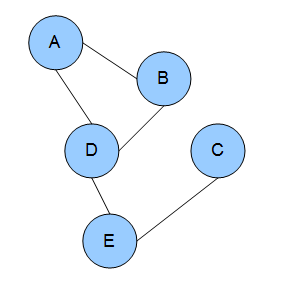
\includegraphics[width=0.4\textwidth]{src/images/mrf-example.png}
  \caption[Example of Markov random fields]{Example of Markov random fields\protect\footnotemark}
  \label{fig:markov}
\end{figure}
\footnotetext{Source (accessed 03/2016): \url{https://en.wikipedia.org}.}

\subsubsection{Dynamic programming}

In general dynamic programming means having a method for an optimization problem to be minimized which can be parted into smaller chunks.
Then these chunks get solved individually and in the end the optimization problem is minimized \citep{angel1972dynamic, bellman2015applied, cyganek2011introduction}.
For stereo matching this applies to the partition of a two-dimensional search problem into a series of isolated one-dimensional search problems on each pair of epipolar lines.
These problems are then solved independently.
With dynamic programming the following energy function (introduced in the foundations chapter \ref{chap:foundations} can be solved independently per scanline.

\begin{equation}
  E(d) = E_{data}(d) + \lambda E_{smooth}(d)
\end{equation}

%todo more
Blabla \citep{cyganek2011introduction}.

\subsubsection{Belief propagation}

Belief propagation is in general a technique to perform inference on a probabilistic model like Bayesian networks or Markov random fields.
Key part of belief propagation are factor graphs.

Probabilistic model with Markov random fields. \citep{yedidia2003understanding}

\begin{itemize}
  \item Define factor graphs
  \item Link to Bayesian network.
  \item Link to Markov random fields.
  \item Maybe small explanation of how the sampling procedure to obtain the maximum works.
\end{itemize}

Belief propagation.
\citep{tappen2003comparison}.

\subsubsection{Graph cuts}

\begin{itemize}
  \item Explain the problem! \citep{boykov2001fast}
  \item Define a graph.
  \item Show the use of a graph in computer vision.
  \item Explain the $\alpha$-$\beta$-swap algorithm.
  \item Explain the $\alpha$-expansion algorithm.
\end{itemize}

Graph cuts.
%todo massage me
Citation \citep{boykov2001fast} develops the graph-cuts algorithms (alpha-expansion and the swap algorithms), citation \citep{ramin2004energy} gives a simpler graph construction for the methods described in \citep{boykov2001fast}, and citation \citep{kolmogorov2004energy} gives an efficient min-cut/max-flow algorithm for computing the minimum graph cut.

\section{Spatiotemporal consistency}

As mentioned in the section before no real disparity algorithm for videos exists yet.
However a novel approach was presented by \citep{richardt2010real}, \citep{khoshabeh2011spatio} and \citep{hosni2012temporally}.

Explain how the video restoration algorithms work (basically). They added noise. Blablabla.

\begin{itemize}
  \item Small description what is currently available.
  \item What can we do?
  \item Explain why some stuff is not available at all.
  \item Also point out the lack of ground truth data. This is a huge problem.
  \item Link to datasets!
\end{itemize}

